\section{Ejercicios propuestos}

\subsection{Ejercicio 1}

En este ejercicio se pide modelizar el ejemplo clásico de la Membrana de Cook, describiéndose su geometría en la Fig.~\ref{figu120} (en mm). La membrana está empotrada en un extremo y sometido a esfuerzo cortante en el opuesto. El esfuerzo aplicado es $F=1.8\ kN$, repartido a lo largo del lado derecho. Las propiedades elásticas del material son $E=70\ GPa$ y $\nu=0.33$, y su espesor es 1 mm. Trabajaremos bajo la hipótesis de tensión plana.
La malla será de tipo estructurada, subdividiendo en 16 partes cada lado del contorno. Se utilizarán el mismo tipo de elemento que en la práctica principal. 
\begin{figure}[!h]
  \begin{center}
    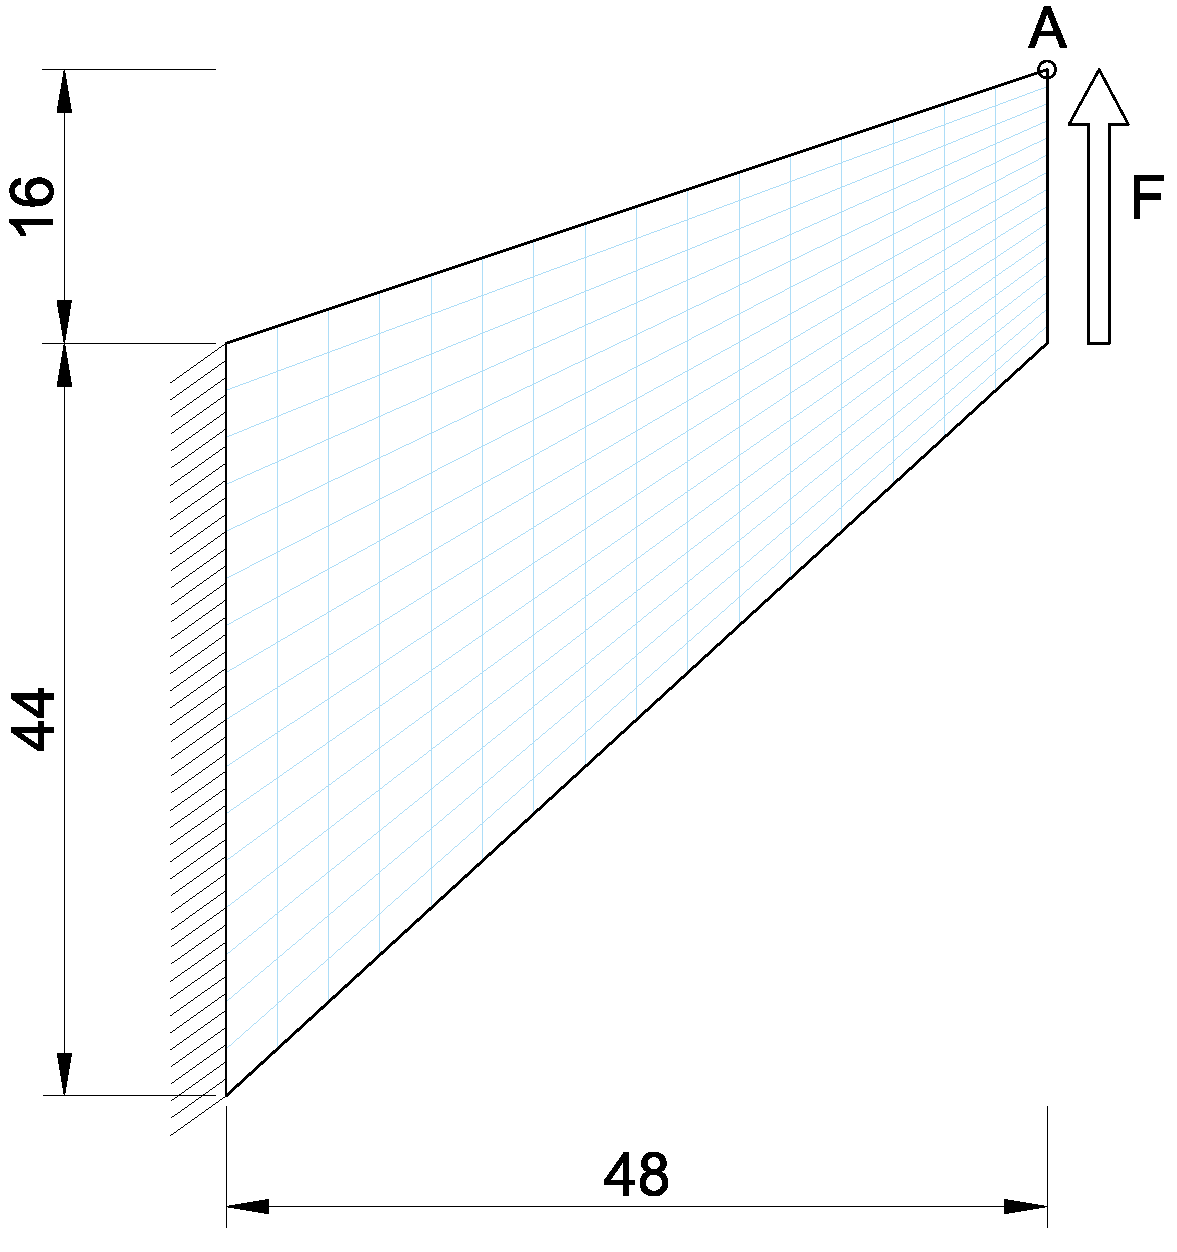
\includegraphics[width=0.55\textwidth]{./body/images/membrana1}
  \end{center}
  \caption{Descripción del modelo}
  \label{figu120}
\end{figure}
\begin{enumerate}
\item ¿Cuál es el módulo del desplazamiento del punto A?
  \begin{multicols}{4}
  \mybox{A: 0.807 mm} %ok$
\columnbreak
\mybox{B: 1.125 mm}
\columnbreak
\mybox{C: 0.689 mm}
\columnbreak
\mybox{D: 1.333 mm}
  \end{multicols}
\item El valor máximo de la reacción en el empotramiento es:
  \begin{multicols}{4}
\mybox{A: 1203.0 N}
\columnbreak
\mybox{B: 857.6 N} %ok$
\columnbreak
\mybox{C: 560.3 N}
\columnbreak
\mybox{D: 251.6 N}
  \end{multicols}
\item El valor máximo de la tensión de Von Mises es:
  \begin{multicols}{4}
\mybox{A: 1321.0 MPa}
\columnbreak
\mybox{B: 854.2 MPa} %ok$
\columnbreak
\mybox{C: 1598.3 MPa}
\columnbreak
\mybox{D: 381.6 MPa}
\end{multicols}
\end{enumerate}


\newpage
\subsection{Ejercicio  2}
A continuación se muestra un ejemplo que formalmente es muy similar al
ejercicio resuelto en la sección anterior. Se trata de una pieza en L
que está empotrada en uno de sus extremos y hay una fuerza repartida
en la mitad de su borde superior. La Fig.~\ref{figu115} resume el
ejemplo.

\begin{figure}[!h]
  \begin{center}
    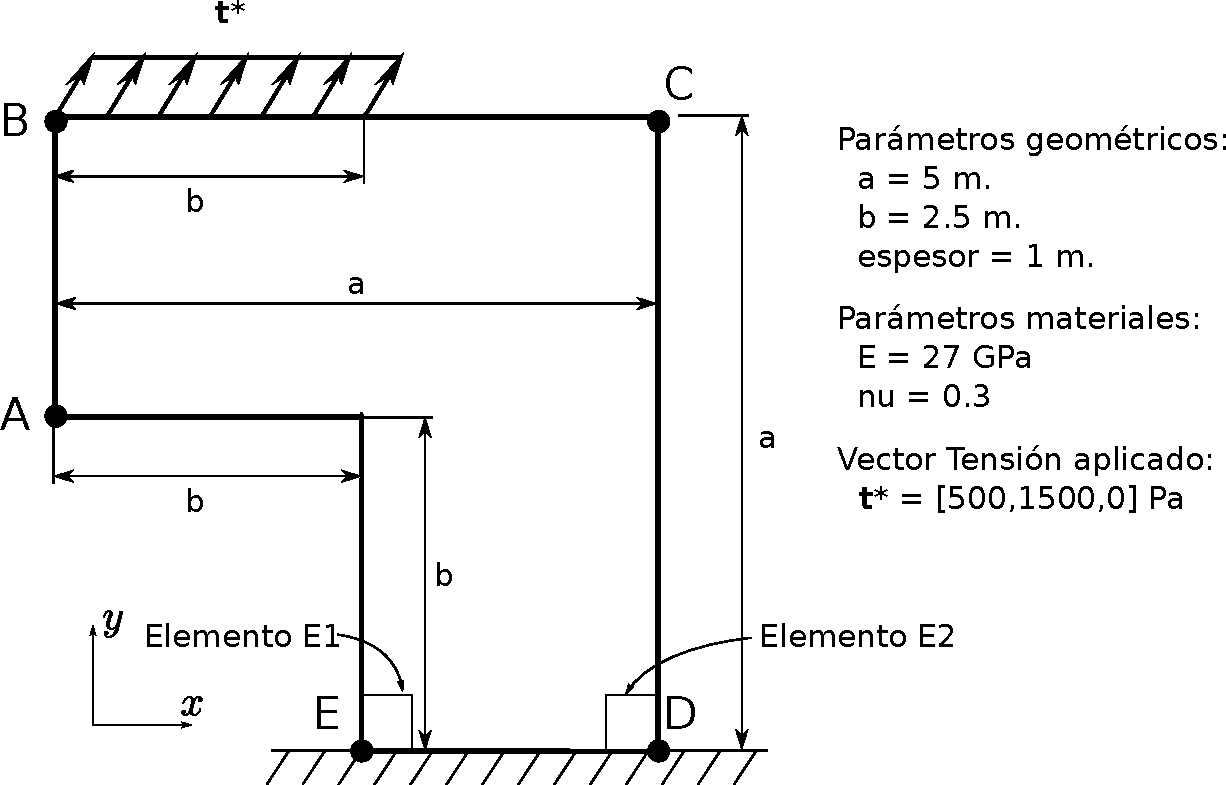
\includegraphics[width=0.65\textwidth]{./body/images/imagen115}
  \end{center}
  \caption{Descripción del modelo}
  \label{figu115}
\end{figure}

Para este modelo, siguiendo el esquema de trabajo de la Sección 1,
utilizando el mismo tipo de elemento cuadrilátero y un tamaño global
de elemento de valor $0.3$ metros, responde las siguientes preguntas:


\begin{enumerate}
\item ¿Cuál es el desplazamiento vertical del punto B?
\begin{multicols}{4}
\mybox{A: 2.821 $\cdot$ 10$^{-6}$ m.}
\columnbreak
\mybox{B: 6.024 $\cdot$ 10$^{-6}$ m.} %OK
\columnbreak
\mybox{C: 2.123 $\cdot$ 10$^{-5}$ m.}
\columnbreak
\mybox{D: 3.254 $\cdot$ 10$^{-9}$ m.}
\end{multicols}
\item ¿Cul es el desplazamiento horizontal del punto C?
\begin{multicols}{4}
\mybox{A: 1.627 $\cdot$ 10$^{-6}$ m.}
\columnbreak
\mybox{B: 4.741 $\cdot$ 10$^{-6}$ m.} %OK
\columnbreak
\mybox{C: 2.321 $\cdot$ 10$^{-5}$ m.}
\columnbreak
\mybox{D: 5.237 $\cdot$ 10$^{-9}$ m.}
\end{multicols}
\item ¿Cuál es la componente $\sigma_{22}$ del tensor de tensiones en el 
centroide del elemento $E1$?
\begin{multicols}{4}
\mybox{A: 1782 Pa.}
\columnbreak
\mybox{B: 17413 Pa.}
\columnbreak
\mybox{C: 7174 Pa.}
\columnbreak
\mybox{D: 14904 Pa.} %OK
\end{multicols}
\item ¿Cuál es el valor máximo (en valor absoluto) de la tensión principal
mínima $\sigma_3$ en el camino $EC$?
\begin{multicols}{4}
\mybox{A: -851 Pa.}
\columnbreak
\mybox{B: -8801 Pa.}
\columnbreak
\mybox{C: -1984 Pa.}
\columnbreak
\mybox{D: -3366 Pa.}%OK
\end{multicols}
\end{enumerate}
%\hspace{20mm}\hrulefill$\star$\hrulefill\hspace{20mm}

\newpage

\subsection{Ejercicio  3}

Queremos estudiar el comportamiento mecánico del modelo presentado en la Fig.~\ref{figu116}, donde los segmentos circulares tienen un radio igual a 1 m. La pieza tiene un estado de \textit{tensión plana} con las siguientes condiciones de contorno:
\begin{itemize}
\item Todos los desplazamientos son nulos en el segmento $AB$.
\item En el segmento $EF$ imponemos el valor del desplazamiento $u_x^*=0.01$ m.
\item Hay una fuerza vertical concentrada de valor $F_y=200$ N.
\end{itemize}

El comportamiento material es elástico lineal e isótropo con módulos elásticos  $E=1000000$ Pa.~y $\nu=0.25$. Para construir el problema discreto usamos una malla con los siguientes parámetros: \textit{quad-dominated, quadratic y con un tamaño global de 0.9}.

\begin{figure}[!h]
  \begin{center}
    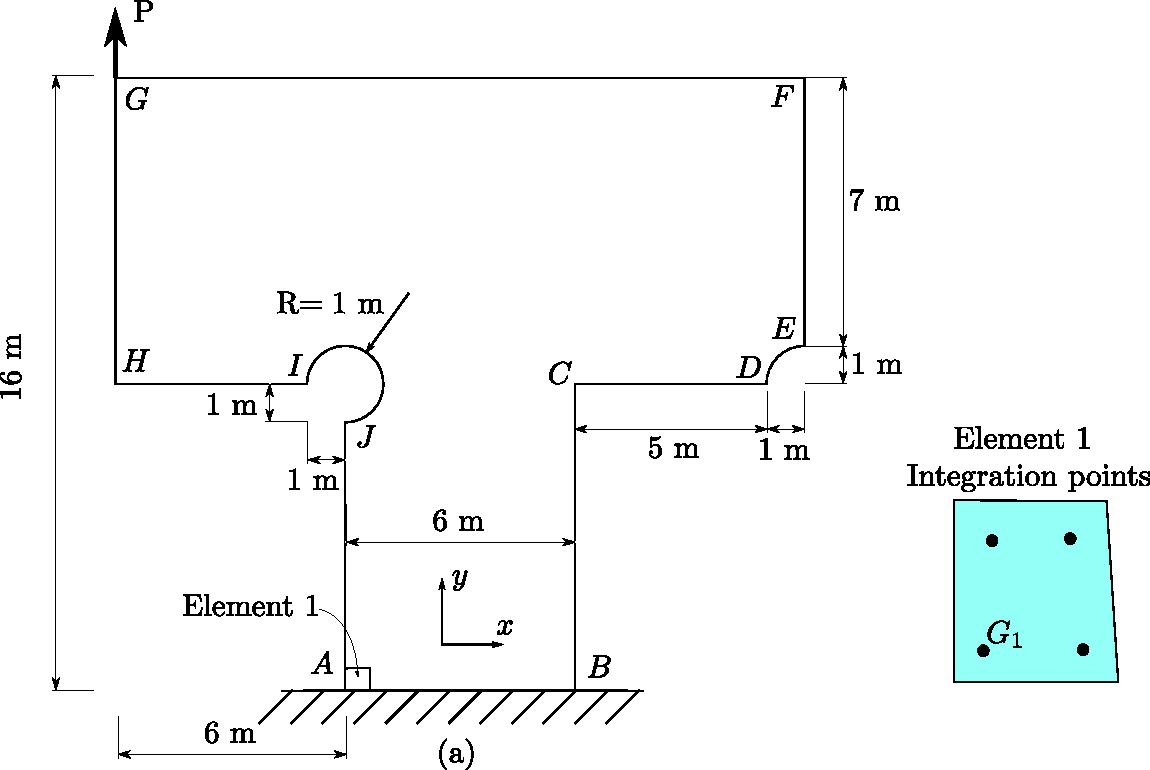
\includegraphics[width=0.65\textwidth]{./body/images/imagen116}
  \end{center}
  \caption{Descriptión del modelo}
  \label{figu116}
\end{figure}

Para este modelo responde las siguientes preguntas  (en este problema debes usar algunos comandos que no hemos explicado en el ejemplo anterior, intenta resolverlo con la ayuda del comando \textit{Help}):



\begin{enumerate}
\item Cuál es el desplazamiento vertical del punto H?
  \begin{multicols}{4}
  \mybox{A: 0.0094 m.} %ok$
\columnbreak
\mybox{B: 0.0025 m.}
\columnbreak
\mybox{C: 0.0125 m.}
\columnbreak
\mybox{D: 0.0003 m.}
  \end{multicols}
\item Cuál es el desplazamiento horizontal del punto J?
  \begin{multicols}{4}
\mybox{A: 0.0012 m.}
\columnbreak
\mybox{B: 0.0050 m.} %ok$
\columnbreak
\mybox{C: 0.0006 m.}
\columnbreak
\mybox{D: 0.0181 m.}
  \end{multicols}
\item Cuál es la componente $\sigma_{22}$ del tensor de tensiones en el punto de integración $G_1$ del elemento 1 (ver figura)?
  \begin{multicols}{4}
  \mybox{A: 710 Pa.} %ok$
\columnbreak
\mybox{B: 1412 Pa.}
\columnbreak
\mybox{C: 172 Pa.}
\columnbreak
\mybox{D: 904 Pa.}
  \end{multicols}
\item Cuál es el valor máximo de la tensión principal máxima en el camino $AF$?
  \begin{multicols}{4}
   \mybox{A: 51 Pa.}
\columnbreak
\mybox{B: 894 Pa.} %ok$
\columnbreak
\mybox{C: 1384 Pa.}
\columnbreak
\mybox{D: 323 Pa.}
\end{multicols}
\item Cuál es la suma de las fuerzas de reacción horizontales en la base $AB$?
  \begin{multicols}{4}
   \mybox{A: -231.75 N.}%ok
\columnbreak
\mybox{B: -124.87 N.}
\columnbreak
\mybox{C: -13 N.}
\columnbreak
\mybox{D: -323 N.}
  \end{multicols}
\end{enumerate}
%\hspace{20mm}\hrulefill$\star$\hrulefill\hspace{20mm}

